% !TEX encoding = UTF-8 Unicode
%%%%%%%%%%%%%%%%%%%%%%%%%%%%%%%%%%%%%%%%%
% Seminário
% LaTeX Template
% Version 1.0 (13/03/19)
%
% Author: Fred Guth (fredguth@fredguth.com)
%
% License:
% CC BY-NC-SA 3.0 (http://creativecommons.org/licenses/by-nc-sa/3.0/)
%
%%%%%%%%%%%%%%%%%%%%%%%%%%%%%%%%%%%%%%%%%

%----------------------------------------------------------------------------------------
%	PACKAGES AND OTHER DOCUMENT CONFIGURATIONS
%----------------------------------------------------------------------------------------

\documentclass[
10pt, % Default font size is 10pt, can alternatively be 11pt or 12pt
a4paper, % Alternatively letterpaper for US letter
onecolumn, % Alternatively twocolumn
% portrait % Alternatively landscape
]{article}

%%%%%%%%%%%%%%%%%%%%%%%%%%%%%%%%%%%%%%%%%
% Paper Notes
% Structure Specification File
% Version 1.0 (25/10/18)
%
% Author: Fred Guth (fredguth@fredguth.com
%
% License:
% CC BY-NC-SA 3.0 (http://creativecommons.org/licenses/by-nc-sa/3.0/)
%
%%%%%%%%%%%%%%%%%%%%%%%%%%%%%%%%%%%%%%%%%%%%%%%%%%%%%%%%%%%%%%%%%%%%%%%%%%%%%%%%%%

%----------------------------------------------------------------------------------------
%	REQUIRED PACKAGES
%----------------------------------------------------------------------------------------

\usepackage[includeheadfoot,columnsep=2cm, left=1in, right=1in, top=.5in, bottom=.5in]{geometry} % Margins

\usepackage[utf8]{inputenc}
\usepackage{XCharter} % XCharter as the main font
\usepackage{booktabs}
\usepackage{natbib} % Use natbib to manage the reference
\usepackage{bibentry}
\usepackage{amsmath}
\usepackage{amsthm}
\usepackage{graphicx, wrapfig}
\graphicspath{ {./imgs/} }

\nobibliography*
\bibliographystyle{plain} % Citation style

\usepackage[brazil]{babel} % Use english by default

%----------------------------------------------------------------------------------------
%	CUSTOM COMMANDS
%----------------------------------------------------------------------------------------
\newcommand{\horrule}[1]{\rule{\linewidth}{#1}} % Create horizontal rule command with 1 argument of height
\newcommand{\papertitle}[1]{\renewcommand{\papertitle}{#1}} % Define a command for storing the article title
\newcommand{\papercitation}[1]{\renewcommand{\papercitation}{#1}} % Define a command for storing the article citation
\newcommand{\lectureabstract}[1]{\renewcommand{\lectureabstract}{#1}}
% \newcommand{\doctitle}{``\papertitle''\---\papercitation  } % Define a command to store the article information as it will appear in the title and header

\newcommand{\datenotesstarted}[1]{\renewcommand{\datenotesstarted}{#1}} % Define a command to store the date when notes were first made
\newcommand{\docdate}[1]{\renewcommand{\docdate}{#1}} % Define a command to store the date line in the title

\newcommand{\docauthor}[1]{\renewcommand{\docauthor}{#1}} % Define a command for storing the article notes author

% Define a command for the structure of the document title
\newcommand{\printtitle}{

\begin{center}

  \horrule{0.5pt} \\[0.4cm] % Thin top horizontal rule

  \bigskip

  \textbf{\Large{"\papertitle"}}
  
  \bigskip
  \begin{minipage}{.9\textwidth}
  \lectureabstract
  \end{minipage}
  \bigskip
  
  \docdate

  \docauthor

  \bigskip
  

  \horrule{2pt} \\[0.5cm] % Thick bottom horizontal rule

\end{center}


}

%----------------------------------------------------------------------------------------
%	STRUCTURE MODIFICATIONS
%----------------------------------------------------------------------------------------

\setlength{\parskip}{3pt} % Slightly increase spacing between paragraphs

% Uncomment to center section titles
%\usepackage{sectsty}
%\sectionfont{\centering}

% Uncomment for Roman numerals for section numbers
%\renewcommand\thesection{\Roman{section}}
 % Input the file specifying the document layout and structure
%----------------------------------------------------------------------------------------
%	ARTICLE INFORMATION
%----------------------------------------------------------------------------------------

\papertitle{Uma Breve Introdução à Teoria da Aprendizagem Computacional} % The title of the article
               
\datenotesstarted{12 de março de 2019} % The date when these notes were first made
\docdate{\datenotesstarted; rev. \today} % The date when the notes were lasted updated (automatically the current date)

\docauthor{Fred Guth} % Your name

%----------------------------------------------------------------------------------------

\begin{document}

\pagestyle{myheadings} % Use custom headers
\markright{\papertitle} % Place the article information into the header

%----------------------------------------------------------------------------------------
%	PRINT ARTICLE INFORMATION
%----------------------------------------------------------------------------------------

\thispagestyle{plain} % Plain formatting on the first page

\printtitle % Print the title

%----------------------------------------------------------------------------------------
%	ARTICLE NOTES
%----------------------------------------------------------------------------------------

\section*{Preâmbulo} 

    Complexidade Computacional, que aqui na UnB vemos no curso de Projeto e Complexidade de Algoritmos é um dos alicerces de qualquer curso de Ciência da Computação. A ideia desse campo de estudo é examinar e classificar problemas de acordo com sua dificuldade de solução (P vs NP, por exemplo). Ao fazer esse curso no semestre passado e tendo como área de interesse aprendizado de máquinas, me perguntei: Será que não seria possível trazer esses conceitos de complexidade de algoritmos para aprendizado de máquinas, analisando qual seria a quantidade de amostras necessárias para um algoritmo aprender uma tarefa?

    A resposta é sim. Essa ideia não é, obviamente, original. Em 1984, Leslie Valiant publicou o modelo de aprendizado "Provavelmente Aproximadamente Correto" (PAC, Probably Approximately Correct), justamente com o objetivo de incitar pesquisadores que estudavam complexidade de algoritmos a pensar problemas de aprendizado.  Ele introduziu a ideia de problemas de aprendizado que são apreensíveis em tempo polinomial, PAC apreensíveis, em analogia com a classe dos problemas P. Pode-se dizer que foi bem sucedido:  diversos pesquisadores estenderam ou propuseram novas teorias, o que originou o ramo de estudo chamado de Teoria de Aprendizado Computacional, que tem até a sua própria conferência anual, COLT (Conference on Learning Theory).
    
    Nesta apresentação meu objetivo é apresentar o modelo PAC, contextualizar a Teoria do Aprendizado na minha linha de pesquisa e me colocar a disposição de alunos e professores interessados para discutir mais este assunto.

%------------------------------------------------

\section*{O que é Apreensível?}

O que é apreensível? Essa é uma questão muito anterior à Ciência da Computação.  No século 18, o filósofo escocês David Hume se perguntou se é possível gerar conhecimento a partir da indução (O problema da Indução).  O que é justamente a base do aprendizado supervisionado, a área da Inteligência Artificial mais pesquisada no momento.  

Para Hume, não há justificativa lógica para generalizações baseadas em indução. Por exemplo: "Sempre que no passado comi pão, ele me alimentou. O futuro será como o passado. Portanto, da próxima vez que comer pão ele me alimentará.", não tem justificativa.  Para ele nós vemos causalidade onde há apenas a conjunção constante entre dois acontecimentos distintos. Mas se isso é verdade, é possível obter conhecimento através da indução?  E se não é possível, o aprendizado indutivo supervisionado não tem justificativa? Pior, o método científico não pode ser logicamente justificado?

A abordagem de Valiant traz uma resposta ao mesmo tempo prática e formal para esse problema.  Não é possível dizer que "esse pão que ainda não comi vai me alimentar", sem comê-lo. Entretanto, é possível dizer, com certo nível de confiança que a hipótese "vai me alimentar" está aproximadamente correta. Em outras palavras, embora seja possível que o pão não me alimente (vai que está estragado?), na maioria das vezes ele me alimenta e é possível mensurar a probabilidade desta hipótese estar aproximadamente correta. 

Confuso? Vamos colocar mais matemática nessa discussão para deixar tudo mais claro. Só que antes, algumas definições.


%------------------------------------------------

\section*{Aprendizado-PAC: Definições}

Genericamente, podemos pensar em um algoritmo como uma função que transforma uma  instância do espaço de entrada, $\mathcal{X}$, em uma instância do espaço de soluções da tarefa que queremos realizar, $\mathcal{Y}$. Em geral, essa função é um conjunto de regras programadas.

\begin{figure}[!htp]
    \centering
    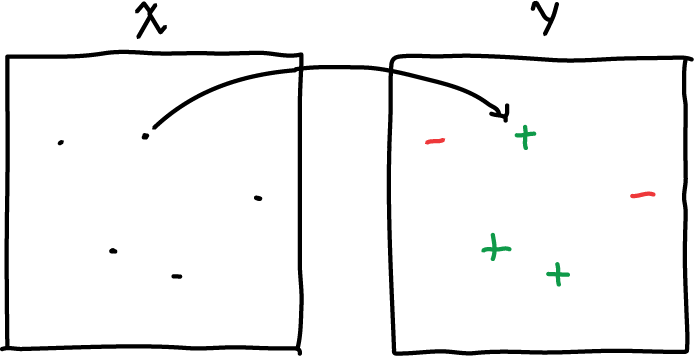
\includegraphics[width=.8\textwidth]{function}
    \label{function}
    \caption{Um algoritmo genérico: $\mathcal{X} \to \mathcal{Y}$.}
\end{figure}

No contexto de aprendizado de máquina, não sabemos expressar essa função alvo, portanto teremos que inferi-la, aprendê-la. Chamaremos essa função ideal de \emph{conceito}. É o conceito que queremos aprender.

\begin{figure}[!htp]
    \centering
    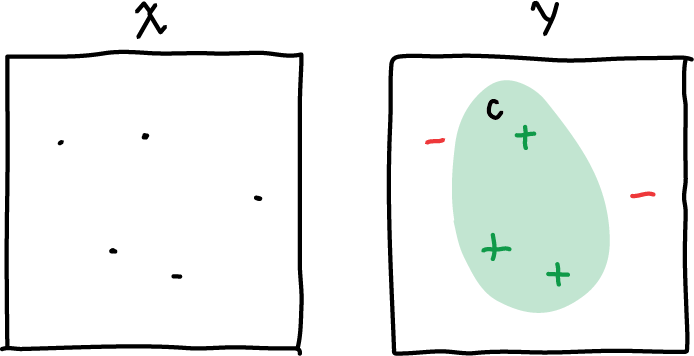
\includegraphics[width=.8\textwidth]{concept}
    \label{concept}
    \caption{Um conceito $c$.}
\end{figure}

A função realmente obtida, a regra, a heurística, chamamos de \emph{hipótese}. Uma hipótese pertence a um espaço de Hipóteses: $h \in \mathcal{H}$.
\begin{figure}[!htp]
    \centering
    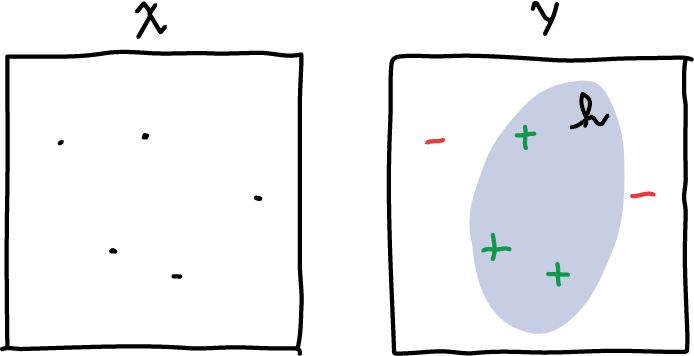
\includegraphics[width=.8\textwidth]{hypothesis}
    \label{hypothesis}
    \caption{Uma hipótese $h \in \mathcal{H}$.}
\end{figure}

  
\begin{figure}[!htp]
    \centering
    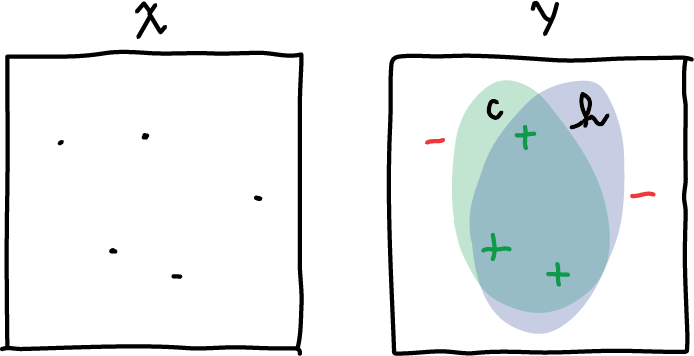
\includegraphics[width=.8\textwidth]{conceptVShypothesis}
    \label{conceptVShypothesis}
\end{figure}

%
%----------------------------------------------------------------------------------------
%
%----------------------------------------------------------------------------------------
%	BIBLIOGRAPHY
%----------------------------------------------------------------------------------------

\renewcommand{\refname}{References} % Change the default bibliography title

\bibliography{references} % Input your bibliography file

%----------------------------------------------------------------------------------------

\end{document}